
\subsection{Simulation des Grandes Échelles}

$$
\frac{\partial\bar{\rho}}{\partial t}+\frac{\partial\bar{\rho}\tilde{u_j}}{\partial x_j}=0
$$

\begin{equation}
    \dfrac{\partial \bar\rho \tilde{u}_i}{\partial t} + \dfrac{\partial \bar\rho \tilde{u}_i\tilde{u}_j}{\partial x_j} + \dfrac{\partial \bar p}{\partial x_i} - \dfrac{\partial \overset{\smile}{\sigma}_{ij}}{\partial x_j} = -\dfrac{\partial \tau_{ij}}{\partial x_j} + \dfrac{\partial}{\partial x_j} \left( \overline{\sigma_{ij}} - \overset{\smile}{\sigma}_{ij}\right),
    \label{eq:les_momentum_eqns}
\end{equation}

$$
 \frac{\partial \bar{\rho} \tilde{E}}{\partial t}+\frac{\partial(\bar{\rho} \tilde{E}+\bar{p}) \tilde{u}_j}{\partial x_j}-\frac{\partial \overset{\smile}{\sigma}_{i j} \tilde{u}_i}{\partial x_j}+\frac{\partial \overset{\smile}{q}_j}{\partial x_j} \\
 =-\frac{\partial}{\partial x_j}\left[C_p Q_j+\mathcal{J}_j-\mathcal{D}_j-\left(\overline{q_j}-\overset{\smile}{q}_j\right)\right] .
$$
where the $\tilde{\cdot}$ overset denotes Favre averaging, the $\bar\cdot$ overset denotes Reynolds averaging, and $\overset{\smile}{\sigma}_{ij}$ depends on the computable rate-of-strain tensor:

\begin{equation}
    \overset{\smile}{\sigma}_{ij} = \mu(\tilde{T}) \left( 2 \tilde{S}_{ij} - \dfrac{2}{3}\delta_{ij}\tilde{S}_{kk} \right),~~ \tilde{S}_{ij} = \dfrac{1}{2}\left( \dfrac{\partial\tilde{u}_i}{\partial x_j} + \dfrac{\partial \tilde{u}_j}{\partial x_i}\right).
    \label{eq:sigma_smile}
\end{equation}

All overset variables are computable whereas we need a closure for the subgrid-scale stress tensor $\tau_{ij}$.
In HYPERION, we follow a Boussinesq type hypothesis \cite{boussinesq1877essai} that leads to the subgrid-scale stress tensor having the following mathematical form:

\begin{equation}
    \tau_{ij} - \dfrac{1}{3}\delta_{ij}\tau_{kk} = - 2 \bar\rho \nu_{\text{sgs}} \left( \tilde{S}_{ij} - \dfrac{1}{3} \delta_{ij}\tilde{S}_{kk} \right),
    \label{eq:boussinesq_les}
\end{equation}

The SGS temperature flux is defined:

$$Q_j = \bar{\rho}\left(\overset{\sim}{u_j T} -\tilde{u}_j\tilde T\right)$$

The SGS viscous diffusion is defined:

$$D_j = \bar{\tau_{ij}u_j} - \tilde{\tau}_{ij}\tilde{u}_j $$

The SGS turbulent diffusion is defined:

$$j_j = \frac{1}{2}(\bar{\rho}\overset{\sim}{u_i u_j u_j} - \bar{\rho}\tilde{u}_i \tilde{u}_j \tilde{u}_j -\tau_{sgs_{jj}})$$

\begin{figure}[h!]
 \centering
 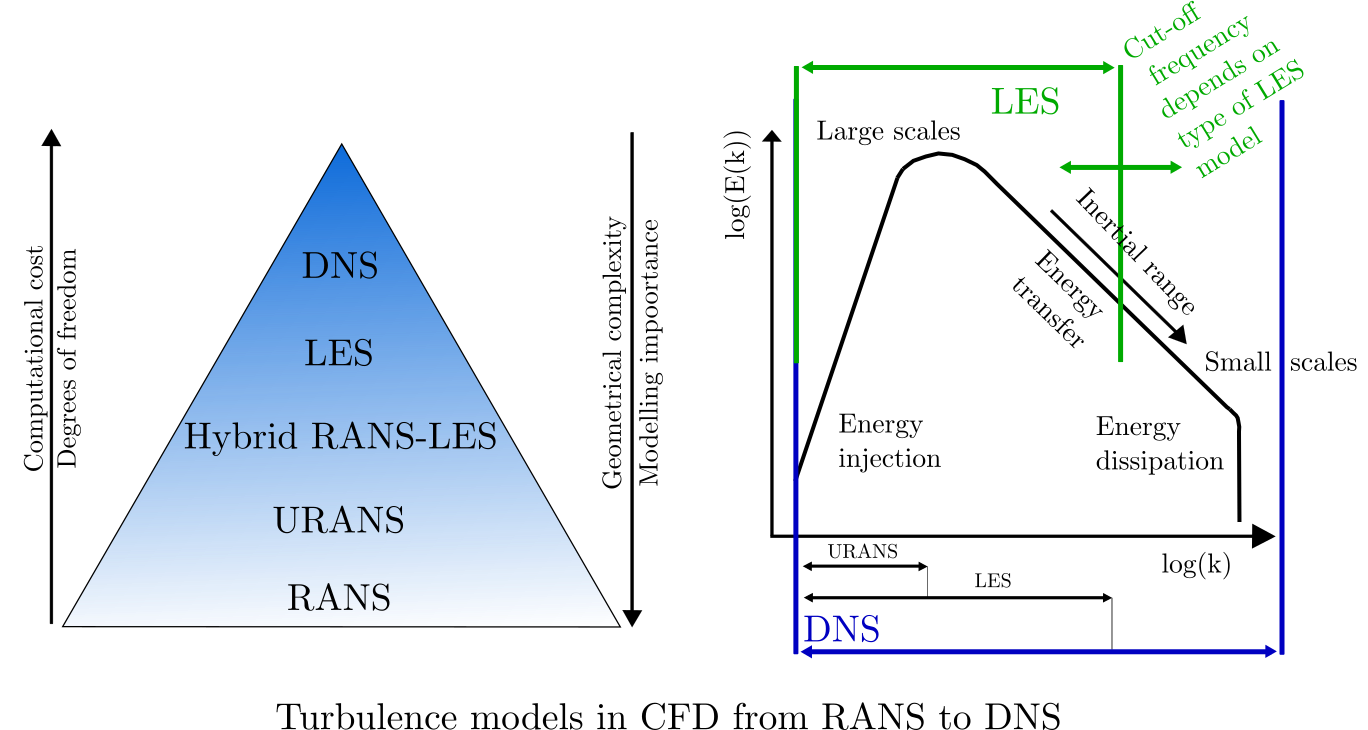
\includegraphics[width=0.7\linewidth]{chapter1_introduction/pictures/les.png}
 \vspace{-2ex}
 \caption{IXV spatial navette by esa}
  \vspace{2ex}
 \label{les}
\end{figure}
